%% Based on a TeXnicCenter-Template by Gyorgy SZEIDL.
%%%%%%%%%%%%%%%%%%%%%%%%%%%%%%%%%%%%%%%%%%%%%%%%%%%%%%%%%%%%%
%
%------------------------------------------------------------
%
\documentclass[a4paper,12pt,reqno]{article}
%----------------------------------------------------------
\usepackage{amsfonts}
\usepackage{graphicx}
\usepackage{geometry}
\usepackage{color}
\usepackage{amssymb,amsmath}
\usepackage{polski}
\usepackage[T1]{fontenc}
\usepackage[utf8]{inputenc}
\usepackage{caption}
\geometry{margin=1.1in}
\usepackage{wrapfig}
\usepackage{lipsum}  
\usepackage{listings}
\usepackage[toc,page]{appendix}
\usepackage{url}

\definecolor{codegreen}{rgb}{0.5, 0.09, 0.09}
\definecolor{codegray}{rgb}{0.5,0.5,0.5}
\definecolor{codepurple}{rgb}{0.58,0,0.82}
\definecolor{backcolour}{rgb}{0.94,0.94,0.94}
\definecolor{gray}{rgb}{0,0.6,0}

\lstdefinestyle{mystyle}{
    backgroundcolor=\color{backcolour},  
    commentstyle=\color{codegreen},
    keywordstyle=\color{blue},
    numberstyle=\tiny\color{codegray},
    stringstyle=\color{codepurple},
		basicstyle=\footnotesize\fontfamily{cmtt}\selectfont,
    breakatwhitespace=false,         
    breaklines=true,
    captionpos=b,
		language=C++,
    keepspaces=true,                 
    numbers=left,                    
    numbersep=5pt,                  
    showspaces=false,                
    showstringspaces=false,
    showtabs=false,                  
    tabsize=2
}
 
\lstset{style=mystyle}
\lstset{literate=%
    *{0}{{{\color{gray}0}}}1
    {1}{{{\color{gray}1}}}1
    {2}{{{\color{gray}2}}}1
    {3}{{{\color{gray}3}}}1
    {4}{{{\color{gray}4}}}1
    {5}{{{\color{gray}5}}}1
    {6}{{{\color{gray}6}}}1
    {7}{{{\color{gray}7}}}1
    {8}{{{\color{gray}8}}}1
    {9}{{{\color{gray}9}}}1
}
%------------------------------------------------------------
\begin{document}

%\begin{figure}[h]
%	\centering
%		
\includegraphics[width=0.40\textwidth]{logo.pdf}
%\end{figure}


\begin{center}

\thispagestyle{empty}

%UNIWERSYTET WROCŁAWSKI\\
\Large 
Uniwersytet Wrocławski\\
Wydział Fizyki i Astronomii\\
\vspace{0.8cm}
\vspace{1.8cm}

\Large Jan Dyplomant \\
\vspace{3.2cm}
\Large Tytuł mojej pracy dyplomowej \\
\vspace{1.5cm}
My diploma thesis title
\end{center}
\vspace{3.7cm}
\begin{flushright}
\large{ Praca magisterska na kierunku \\Fizyka Komputerowa \\}
\large{ Praca inżynierska na kierunku \\Informatyka Stosowana i Systemy Pomiarowe \\}
\vspace{0.5cm}
\large{ Opiekun \\ dr hab. Maciej Matyka, prof. UWr}
\end{flushright}
\vspace{2.2cm}

\begin{center}
\large Wrocław, \today
\end{center}

\newpage

\tableofcontents

\newpage

\begin{flushleft}
\Large \textbf{Streszczenie}
\end{flushleft}
\vspace{1cm}


 Lorem ipsum dolor sit amet, consectetur adipiscing elit, sed do eiusmod tempor incididunt ut labore et dolore magna aliqua. Ut enim ad minim veniam, quis nostrud exercitation ullamco laboris nisi ut aliquip ex ea commodo consequat. Duis aute irure dolor in reprehenderit in voluptate velit esse cillum dolore eu fugiat nulla pariatur. Excepteur sint occaecat cupidatat non proident, sunt in culpa qui officia deserunt mollit anim id est laborum.

\newpage
\begin{flushleft}
\Large \textbf{Abstract}
\end{flushleft}
\vspace{1cm}


Lorem ipsum dolor sit amet, consectetur adipiscing elit, sed do eiusmod tempor incididunt ut labore et dolore magna aliqua. Ut enim ad minim veniam, quis nostrud exercitation ullamco laboris nisi ut aliquip ex ea commodo consequat. Duis aute irure dolor in reprehenderit in voluptate velit esse cillum dolore eu fugiat nulla pariatur.

\newpage

\section{Opis pliku}



W swojej pracy możesz odnosić się do równań np. do równania (\ref{rownanie}) lub do rysunków, zarówno wektorowych, patrz rys. (\ref{logotyp}) jak i bitmapowych (\ref{wahadla}).
Możesz też z powodzeniem cytować literaturę \cite{Sukop, Guo}. Jeśli chcesz to robić wygodniej załóż tzw, plik bibtex, ale możesz też pracować tak, jak w tym dokumencie.
Jesli chcesz wklejać adresu z internetu użyj narzędzia url, np \href{https://youtu.be/GYl3ftE208U}{tak}.


\subsection{Lorem ipsum}

 Lorem ipsum dolor sit amet, consectetur adipiscing elit, sed do eiusmod tempor incididunt ut labore et dolore magna aliqua. Ut enim ad minim veniam, quis nostrud exercitation ullamco laboris nisi ut aliquip ex ea commodo consequat. Duis aute irure dolor in reprehenderit in voluptate velit esse cillum dolore eu fugiat nulla pariatur. Excepteur sint occaecat cupidatat non proident, sunt in culpa qui officia deserunt mollit anim id est laborum.


\newpage
\subsection{Lorem ipsum}
\subsubsection{Lorem ipsum}
 
Lorem ipsum dolor sit amet, consectetur adipiscing elit, sed do eiusmod tempor incididunt ut labore et dolore magna aliqua. Ut enim ad minim veniam, quis nostrud exercitation ullamco laboris nisi ut aliquip ex ea commodo consequat. Duis aute irure dolor in reprehenderit in voluptate velit esse cillum dolore eu fugiat nulla pariatur. Excepteur sint occaecat cupidatat non proident, sunt in culpa qui officia deserunt mollit anim id est laborum.



\begin{equation} 
\rho\left(\frac{\partial\vec v}{\partial t}+(\vec v\cdot\nabla)\vec v\right) =\rho\vec f - \nabla p + \mu\triangle\vec v, \label{rownanie}
\end{equation} 

Lorem ipsum dolor sit amet, consectetur adipiscing elit, sed do eiusmod tempor incididunt ut labore et dolore magna aliqua. Ut enim ad minim veniam, quis nostrud exercitation ullamco laboris nisi ut aliquip ex ea commodo consequat. Duis aute irure dolor in reprehenderit in voluptate velit esse cillum dolore eu fugiat nulla pariatur. Excepteur sint occaecat cupidatat non proident, sunt in culpa qui officia deserunt mollit anim id est laborum.





\begin{figure}[!ht]%
\centering

\includegraphics[scale=0.85]{logo.eps}
\caption{Podpis rysunku, który jest obrazem wektorowym (EPS). \label{logotyp}}
\qquad
\end{figure}   




\begin{figure}[!ht]%
\centering
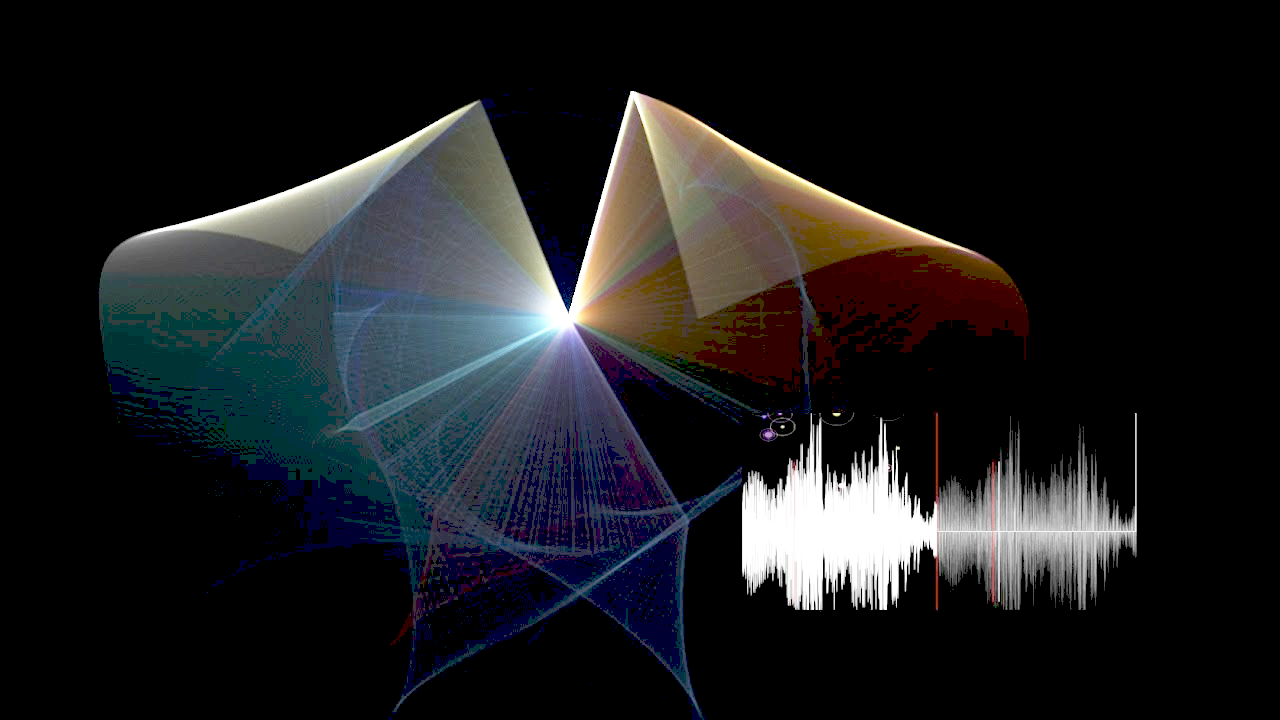
\includegraphics[width=0.8\columnwidth]{pendulums.png}
\caption{To jest rysunek drugi, kilkadziesiąt wahadeł podwójnych z syntezą dźwięku.\label{wahadla}}%
%
\qquad
\end{figure}   



\subsection{Lorem ipsum}

Lorem ipsum dolor sit amet, consectetur adipiscing elit, sed do eiusmod tempor incididunt ut labore et dolore magna aliqua. Ut enim ad minim veniam, quis nostrud exercitation ullamco laboris nisi ut aliquip ex ea commodo consequat. Duis aute irure dolor in reprehenderit in voluptate velit esse cillum dolore eu fugiat nulla pariatur. Excepteur sint occaecat cupidatat non proident, sunt in culpa qui officia deserunt mollit anim id est laborum.
.. in the figure \ref{Rysunek14}.


\newpage

\begin{thebibliography}{2} 

\bibitem{Sukop} T. D. T. J. Sukop, M. C., \textit{Lattice Boltzmann Modeling. An Introduction for Geoscientists and Engineers.} Berlin Heidelberg: Springer-Verlag, 2006.

\bibitem{Guo} Z. Guo, and C. Shu, \textit{Lattice Boltzmann method and its applications in engineering.} World Scientific, 2013.

\bibitem{Adres} Internet: http://www.mit.edu/, data otwarcia: 2019.16.01.

\end{thebibliography}

\end{document}




